\section{File Abstraction}

Our naming scheme is hierarchically structured, like traditional filesystem naming, with support
for symbolic links, allowing arbitrary links between sub-trees.  We argue that this naming scheme
is crucial, as it exposes the inter-relationships which inform aggregation semantics intended
by the user.  We introduce a naming scheme for physical objects and their inter-relationship.


% \vspace{0.08in}


Similar requirements to those aforementioned have been addressed in the design and implementation of filesystems.  Filesystems provide
logical access to physical resources through files, with different files and associated semantics, exposed to applications through a shell
or programmtically.  Filesystems representat collections of bits, encapsulated by a file, and grouped with folders.  Symbolic links support
the notion of multi-naming.  A single file or folder could have multiple names that lead to the same underlying object.  Filesystems even
support the notion of streaming data through character and block device files.  Moreover, pipe files allow programs to communite with each
other through a piece of shared memory, where the source application writes to the pipe and the sink application consumes from the pipe.

We assert that these constructs should be directly adopted for supporting applications in the buildings.  Our approach adopts the unix
file philosophy where everthing is represented as a file.  Each object created in StreamFS is assigned two names, by default, one which 
uniquely identifies the object and \emph{not} human-readable and the second which is changeable and human-readable.  Consider
the example shown in Figure~\cite{fig:everythingfile}.


\begin{figure}[t!] %htbp
\centering
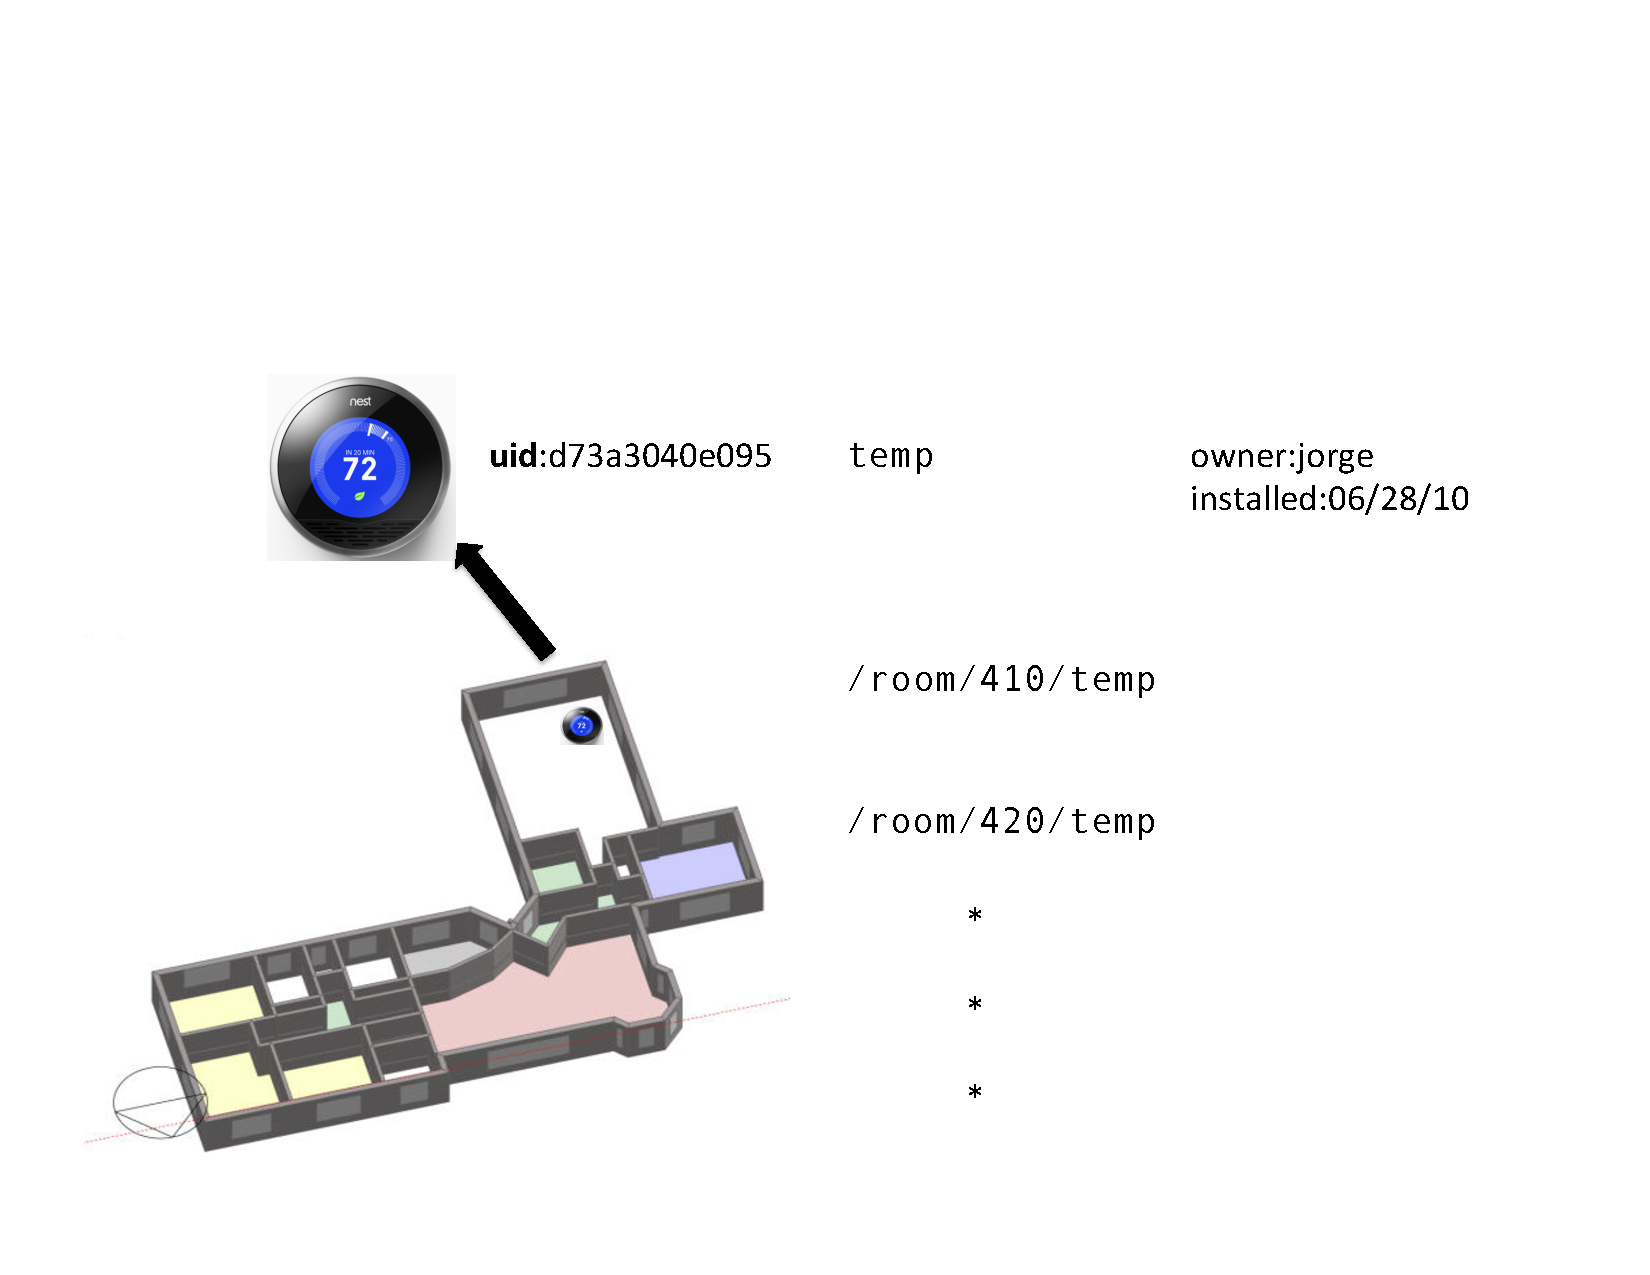
\includegraphics[width=0.65\columnwidth]{figs/everythingfile}
\caption{Everything is a file.  Temperature sensor represented as a file in a folder that contains folders for each room.
Note, the file that represents a temperature sensor producing a stream is given a unique identifer.  The user may also
decorate the file with extra metadata for searching purposes.}
\label{fig:everythingfile}
\end{figure}

In this example, the user is creating a temperature stream file in every room of the building.  The name of the file, given by the user,
is \emph{temp}.  Upon creation, the file is uniquely identified by the system using a unique identifier, as shown.  Like in a unix filesystem, the
file is created within a folder.  Ideally, the name of the folder would encode the placement of the sensor.  In the figure, the 
user is create a temperature stream file in room 410 and room 420.  Note the full filepath for the stream file is /room/410/temp.
During creation, the user may also decorate the file with extra metadata, also shown in the figure.  In this example, they have annotated
the file with information about the owner and when the sensor was installed.   This metadata is used for quickly locating the file
or grouping files that contain similar tags, quickly.

\subsection{File types and operations}
As we map the filesystem abstraction into this problem space, we need to consider the various kinds of files our system will contain,
their semantics, and how our system will expose and manage them.  There are essentially 4 types of files and 6 sub-types.  We summarize
these in Table~\ref{tab:filetypes}.  There are also different kinds of operations that the each file type supports.  Operational semantics
are file dependent.  For example, when you \emph{read} a folder, you obtain the metadata associated with the folder and the name
of its children.  When you \emph{read} a stream, you its metadata and the last timestamp-value it produced.  \emph{Writ}ing to a stream
is a bit different.  You can write to a stream to update its metadata tags and the stream source can write a value to it.  The stream
source is identified with a \emph{publish identifier} (pubid).  The stream source includes the pubid in the write operation for 
the specified stream file.  Without the pubid, the source cannot write to the file.  Any other writer should not be allowed to write to 
a stream file either.  

\begin{table}[h]
\begin{center}
\begin{tabular}{| r | l | l |}
	\hline
	\textbf{type} & \textbf{description} & \textbf{valid operations} \\ \hline
	container & Container file.  Used to group other  & read, write, delete  \\
				   & kinds of files within it.  &  \\ \hline

	stream & Represents a data stream. & read, write, delete, subscribe, \\
			&							&query \\ \hline

	controller & Represents a controller. & read, write, subscribe \\ \hline

	special & There are several kinds of special files for  & read, delete \\
		    & management of jobs and pipes. &  \\ 
	\hline
\end{tabular}
\caption{Summary of the 4 main file types and their valid operations in StreamFS.}
\label{tab:filetypes}
\end{center}
\end{table}

Similar to a traditional filesystem, StreamFS includes \emph{special files}.  There are 6 special files and 5 of them 
are for management purposes.  The only one that is not is the \emph{symbolic link} file, which is essentially used to support
multi-naming and inherents the operational semantics of the file it points to.  The delete operation on a symlink, however,
only deletes the symlink.  A description of these files and the operations they support is given in Table~\ref{tab:filesubtypes}.
A detailed description and examples with be presented in later sections.


\begin{table}[h]
\begin{center}
\begin{tabular}{| r | l | l |}
	\hline
	\textbf{operation} & \textbf{file type} & \textbf{semantics} \\ \hline
	read & folder, stream, ipd, ipi, epd, epi, sub & read the metadata and tags for \\
		 &										   & the associated file. \\ \hline
	write &  stream & Write to stream file, only the \\ 
		  & 		& appropiate stream source is \\
		  &			& permitted.\\ \hline
	delete & folder, stream, ipd, ipi, epd, epi, sub & Folder must be empty.  \\
		   & 										 & The others can be directly deleted. \\ \hline
	query &  stream, all & streams support time-range   \\
		  &			     & queries. All support metadata-tag \\ 
		  &				 & queries. \\ \hline
	subscribe & stream & Forwards data from a stream \\
			  &		   & to the specified destination.\\
	\hline
\end{tabular}
\caption{File opertaitons, the file types that support them, and their general semantics.}
\label{tab:semantics}
\end{center}
\end{table}

\subsection{Container, Stream, and Controller Files}
% \subsection{Default/Folder Files}
A container or folder file serve primarily as a container for other kinds of files.  It is used to group together different kinds of file and
to represent a common attribute of the file within it.  For example, a container file is usually used to construct the spatial hierarchy.
Each file at the top level represents a floor, its children are also a set of container files, representing each of the rooms on that floor.
A container file cannot be deleted unless it is empty (i.e. has no children).

File that represent streams are called stream files.  They are tightly associated with the associated stream data in the timeseries data-store.
A user created a stream file and that associated stream ``writes'' to it in order to have its data saved.  StreamFS also forwards the
data to the \emph{subscription manager} in case any subscription sink has subscribed to this feed.  When a stream file is create an id is 
returned to the user.  This id must be used by the stream that wishes to push its data to StreamFS through this file.  If this id is incorrect
or not include, the write operation is rejected.

Because controllers accpet many kinds of input, we designed the the file that presents a controller similar to the external processing stub discussed
in section~\ref{sec:externalprocs}.  Writes to a controller file and forwarded directly to the control stub running at the controller itself or a proxy
machine that communicates with the controller.  Any reply is set as metadata in the controller file.  Controller files also an associated output stream.
If a controller process wishes to inform the process of internal state at the controller, it does so through the controller file output --
a stream file itself.  Table~\ref{tab:filetypes} lists the files in streamfs and the operations they support.  The operational semantics
are listed in Table~\ref{tab:semantics}.

% \subsection{Stream Files}

% \subsection{Controller Files}

\subsection{Special Files}
There are 6 types of special files.  In chapter~\ref{chap:ProcMngtSchedMain} we eluded to the various kinds of file that are created
when a user creates an internal or external file.  An internal process definition (ipd) file is created when the user
submits a script to StreamFS.  When a (set of) stream(s) is piped through the defintion file, an internal process instance (ipi) file
is created that represents the output of the process.  A subscription instance (sub) file is also created.  The sub file contains
information about which streams are feed the file, a reference to the ipi file, and statistics about the file.  If either
the sub file or the ipi file are deleted, the process ends.  The ipi file is also a stream file.  It can be used to pipe that
output of the process to another processes or to an external \texttt{URL}.

\begin{table}[h]
\begin{center}
\begin{tabular}{| l | l | l |}
	\hline
	\textbf{type} & \textbf{description} & \textbf{valid operations} \\ \hline
	
	internal process  & Javascript process definition.  & read, write, delete  \\ 
	defintion (ipd)   & 							    &	\\ \hline

	internal process  & Management file used for managing & read, delete \\
	instance (ipi)	  & active processing of this script. & \\ \hline

	external process  & Gives information about where an & read, write, delete \\
	definition (epd)  & external process lives. &\\ \hline

	external process  & An active processing stream to an  & read, write, delete \\
	instance (epi)	  & external process. &\\ \hline

	subscription instance & An instance of a subscription.  Contains & read, delete \\
				(sub) 	  & information about the subscription, &\\
								& such as source/sink and related statistics &\\ \hline
								
	symbolic link (symlink) & Similar to a symbolic link in Unix. & \\
	\hline
\end{tabular}
\caption{Summary of the 6 special-file sub-types and their valid operations in StreamFS.}
\label{tab:filesubtypes}
\end{center}
\end{table}

The same set of files are created when an external processes is defined and started.  When the client stub is started on the client
machines it creates an external procrocess definition file for each process that was listed in the configuration file for the stub on 
the client machine.  Similarly, when streams are piped to the defintion files, the client starts the processes on the client
and create their associated external process instance (epi) files.  Those files are also a sub-type of the stream file and can
be used to pipe the output to another process (internal or external) or an external \texttt{URL}.
Any subscription or pipe that is instantiated creates an associated sub file in the \texttt{/sub} directory.  These always contain information
about the subscription and kill the fowarding process when deleted.

Finally, we used symbolic link (symlinks) the same way they are used in a traditional filesystem.  They are also used to generalize
the inter-relationship structure in the ERG.  They are a crucial file in the support of multi-naming.

\subsection{Interfaces}
We built several interfaces to interact with a StreamFS deployment.  Because StreamFS has its own file types and semantics
we created a native shell application and a web-application console.  The web application console is displayed in 
Figure~\ref{fig:sfsconsole}.  The console has various features, all mirrored in the shell application.  It provides
a graphical interface for viewing the files in the deployment, changed the attribute-value pairs associated with file

\begin{figure}[htb!]
\begin{center}
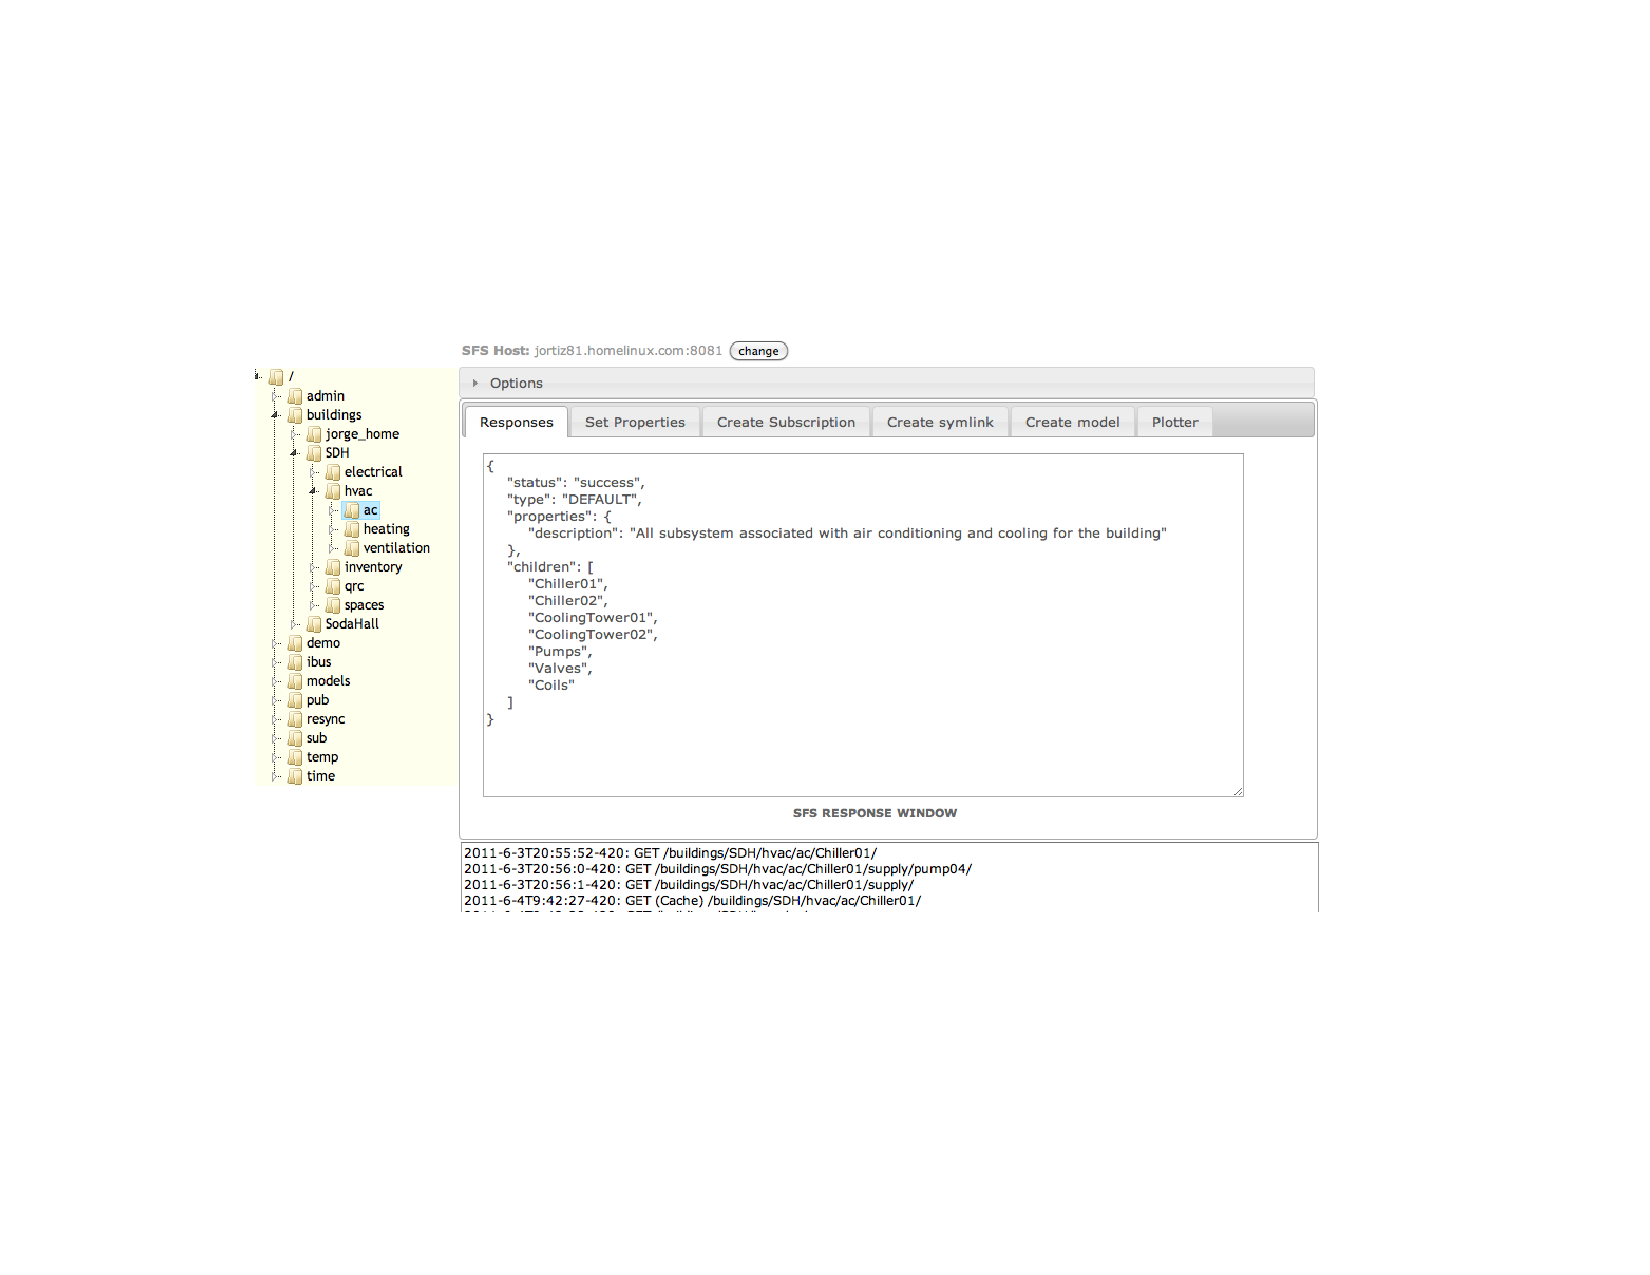
\includegraphics[scale=0.6]{figs/sfs_console}
\caption{StreamFS console.  The tool allows the user to view the namespace as a set of files, interact with the system, and 
view stream data.}
\label{fig:sfsconsole}
\end{center}
\end{figure}

Also available to the user is the ability to create and manage symbolic links, submit small processing jobs, pipe
streams to external target or processing jobs, and plot.  The plotter is a basic mechanism to check if streams are 
active and for exploration purposes.



% \subsection{Special Files}

% \subsubsection{Internal Process Definition}
% \subsubsection{Internal Process Instance}
% \subsubsection{External Process Definition}
% \subsubsection{External Process Instance}
% \subsubsection{Subscription Instance}









